\documentclass[10pt]{article}
\usepackage[spanish]{babel}
\usepackage[utf8]{inputenc}
\usepackage{graphicx}
\usepackage{hyperref}
\usepackage[lmargin=2cm, rmargin=2cm, top=2cm, bottom=2 cm]{geometry}
\usepackage{fancyhdr}
\usepackage[table,xcdraw]{xcolor}
\pagestyle{fancy}
\fancyhead{}
\fancyhead[R]{Página \thepage \hspace{0.02 cm} de 12}
\fancyhead[L]{Tarea N° 01}
\usepackage{animate}
\usepackage{enumerate}
\usepackage{float}
\usepackage{url}
\usepackage{svg}
\usepackage{amsmath}

\hypersetup{ colorlinks, citecolor=black, filecolor=black, linkcolor=black, urlcolor=black }

\usepackage{wrapfig}
\usepackage{subfig}

% Cajas de colores
%Cajas de colores con tcolorbox
%\usepackage{tcolorbox}
\usepackage[most]{tcolorbox}

% markdown readme
\usepackage[hashEnumerators,smartEllipses]{markdown}

% Permitir multi columns
\usepackage{multicol}

%Código para usar script en latex

\usepackage{color}
\usepackage{listings}
\usepackage{adjustbox}

\lstdefinelanguage{Dockerfile}
{
  morekeywords={FROM, RUN, CMD, LABEL, MAINTAINER, EXPOSE, ENV, ADD, COPY,
    ENTRYPOINT, VOLUME, USER, WORKDIR, ARG, ONBUILD, STOPSIGNAL, HEALTHCHECK,
    SHELL},
  morecomment=[l]{\#},
  morestring=[b]"
}

\lstset{
    columns=flexible,
    keepspaces=true,
    showstringspaces=false,
    basicstyle=\tiny\ttfamily,
    commentstyle=\color{gray},
    keywordstyle=\color{purple},
    stringstyle=\color{green}
}



\newcommand{\cabeza}[1]{\noindent{\sc \fbox{#1}}}%Comando para quitar la identación

\renewcommand{\headrulewidth}{0.9pt}
\renewcommand{\footrulewidth}{0.5pt}

% Codigo con colores
\usepackage{minted}
\usemintedstyle{perldoc}


\begin{document}
\date{}  
\begin{titlepage}
\begin{center}
    \vspace*{\baselineskip}
    
    {
    \bf\fontsize{19}{0}{\selectfont{UNIVERSIDAD DIEGO PORTALES}}\\[0.5cm]
    \fontsize{11}{0}{FACULTAD DE INGENIERÍA Y CIENCIAS}
    }
    
    \vspace*{0.5\baselineskip}
    {
    \bf\fontsize{11}{0}{\selectfont{ESCUELA DE INFORMÁTICA Y TELECOMUNICACIONES}}\\[0.35cm]
    }
    
    \vspace*{\baselineskip}
    
\includegraphics[scale=0.30]{logo_udp.png}
    \vspace*{3\baselineskip}
     \hrule height 0.5pt
    \vspace{1mm}
    \hrule height 1.5pt
    \vspace*{1\baselineskip}
   
    {
    \bf\fontsize{15}{0}{\selectfont{Arquitecturas Emergentes \\[0.3cm]Tarea 01: Simulación de redes con Mininet}}
    }
    \vspace*{1\baselineskip}
    \hrule height 0.5pt
    \vspace{1mm}
    \hrule height 1.5pt
    
    
    \vspace*{4.5\baselineskip}
    
    {
     \bf\fontsize{14}{0}{\selectfont{Profesor: Carlos García
}}\\[0.3cm]
   \bf\fontsize{14}{0}{\selectfont{Estudiante: Felipe Condore}}
   }
    
    \vfill
    Santiago, Chile, \hfill Septiembre 2022
    
\end{center}
\end{titlepage}
\vspace*{\baselineskip}
\tableofcontents 
\setcounter{page}{0}
\thispagestyle{empty}
\newpage





\section{Introducción}

\noindent
Uno de los aspectos más importantes en el último tiempo, corresponde a la virtualización de los diversos recursos TI, los cuales no solo corresponden a máquinas computacionales, si no también a diversos componentes que conforman la red. 
\newline

\noindent
Para el siguiente trabajo se lleva a cabo una serie de experimentos a través del Software de Mininet, el cuál nos brinda la posibilidad de simular distintos entornos de una red, a través de un controlador virtual y global, para el manejo del tráfico.
\newline

\noindent
Las pruebas realizadas pretender analizar el comportamiento de diversas acciones en la red, como lo son el establecimiento de un canal de TCP, comunicación mediante pings e intercambio de archivos a través de servicios de FTP, a través de redes cuyas topologías son diseñadas de manera personalizada con parámetros establecidos a través de código.

\section{Configuración de Ambiente}
Para lograr realizar la actividad, es necesario tener en consideración los siguientes requerimientos.

\begin{itemize}
    \item Sistema Operativo: Ubuntu 18.04
    
    \item Docker 20.10.17
    
\end{itemize}

Para poder usar el software de mininet, va a ser necesario ocupar la imagen Containernet que se puede obtener de Docker Hub. Para lograr ciertos requerimientos es necesario crear una propia imagen, tanto de mininet como para los hosts con la finalidad de adquirir ciertas dependencias faltantes. A continuación de presentan los archivos Dockerfile con el cual crear las imágenes para cada equipo, junto a los comandos necesarios para llevar a cabo el despliegue del ambiente.

\begin{multicols}{2}
\begin{figure}[H]
    \centering
    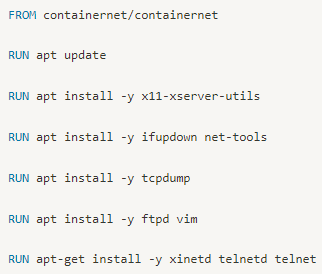
\includegraphics[width=0.8\linewidth]{Imagenes/dockerfile_mininet.png}
    \caption{Imagen de mininet en docker}
    \label{fig:dockerfile_mininet}
\end{figure}

\columnbreak

\begin{figure}[H]
    \centering
    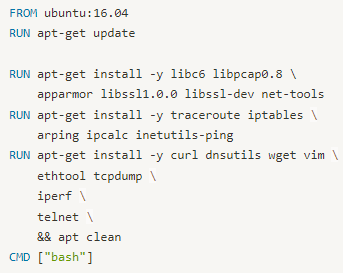
\includegraphics[width=0.8\linewidth]{Imagenes/dockerfile_host.png}
    \caption{Imagen de los host en docker}
    \label{fig:docker_run01}
\end{figure}

\end{multicols}

\begin{figure}[H]
    \centering
    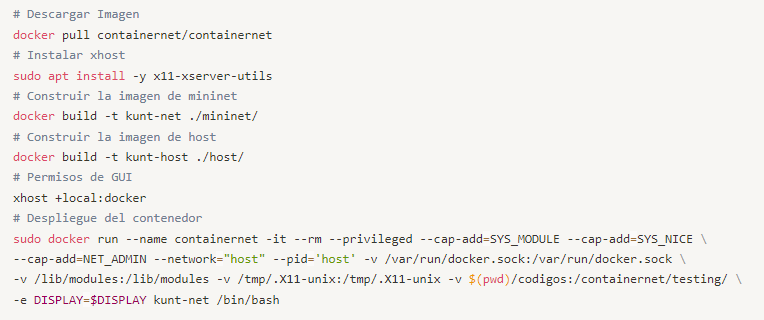
\includegraphics[width=\linewidth]{Imagenes/docker_run.png}
    \caption{Comandos requeridos para el despliegue de Mininet en contenedores}
    \label{fig:dockerrun}
\end{figure}
Una vez dentro del contenedor, antes de realizar cualquiera de las pruebas anteriores, es necesario actualizar la lista de servidores DNS. Para ello pueden ejecutar el script de bash dsn.sh que se encuentra en el directorio /containernet/testing/dns.sh . Este script va a agregar la ip de Google como un servidor DNS extra en la configuración de la máquina, para evitar problemas con la detección de nombres de sitios web públicos.


\section{Experimentos}

\subsection{Actividad 1}

\begin{multicols}{2}
Se lleva a cabo la implementación de la red mostrada en la figura \ref{fig:net01}, a través de un archivo de python. Para realizar esto, dentro del contenedor se utiliza el siguiente comando que permite desplegar la red a través de la topología personalizada.

\columnbreak

\begin{minted}[frame=lines, fontsize=\footnotesize,linenos]{bash}
#!/bin/bash
sudo mn --custom /containernet/testing/pregunta1.py \
--topo mytopo
\end{minted}

\end{multicols}

\begin{figure}[H]
    \centering
    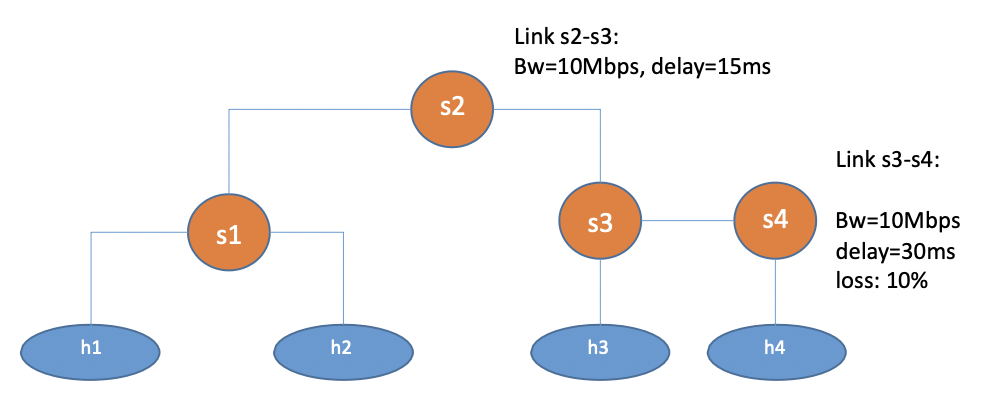
\includegraphics[width=0.6\textwidth]{Imagenes/item01_network.png}
    \caption{Topología de red - Actividad 01}
    \label{fig:net01}
\end{figure}

\noindent
Una vez dentro de la consola de containernet, es posible comprobar los nodos de la red (compuesta por los host y switches), a la vez que se puede obtener las direcciones ip asociadas a cada uno de los host, donde h1, h2, h3 y h4 poseen las direcciones 10.0.0.1, 10.0.0.2, 10.0.0.3 y 10.0.0.4 respectivamente. \newline

\begin{figure}[H]
    \centering
    \subfloat[Configuración de red host h1]{
        \label{CDF11}
        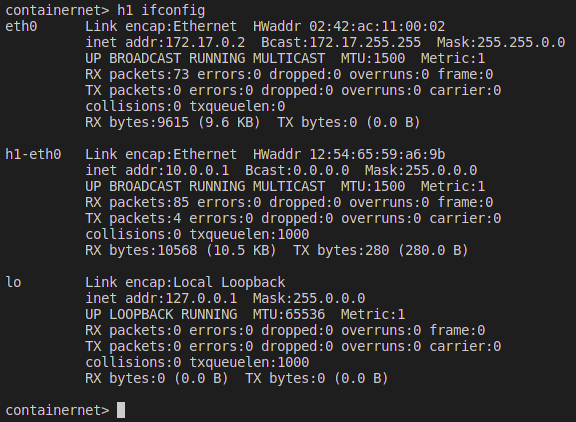
\includegraphics[width=0.45\textwidth]{Imagenes/item01_h1_ifconfig.png}}
    \subfloat[Configuración de red host h2]{
        \label{CDF21}
        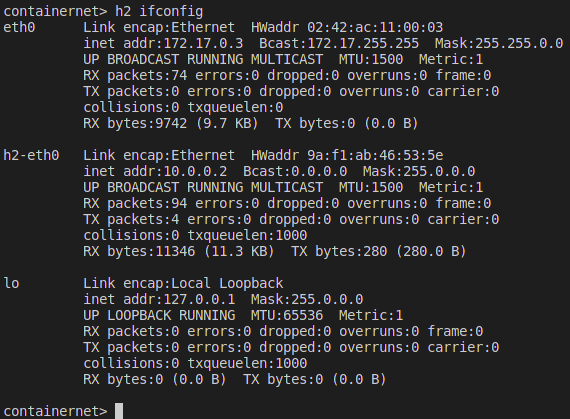
\includegraphics[width=0.45\textwidth]{Imagenes/item01_h2_ifconfig.png}}\\
    \subfloat[Configuración de red host h3]{
        \label{CDF122}
        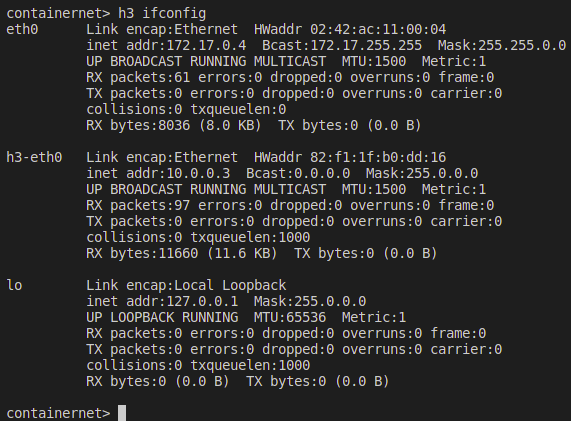
\includegraphics[width=0.45\textwidth]{Imagenes/item01_h3_ifconfig.png}}
    \subfloat[Configuración de red host h4]{
        \label{CDF233}
        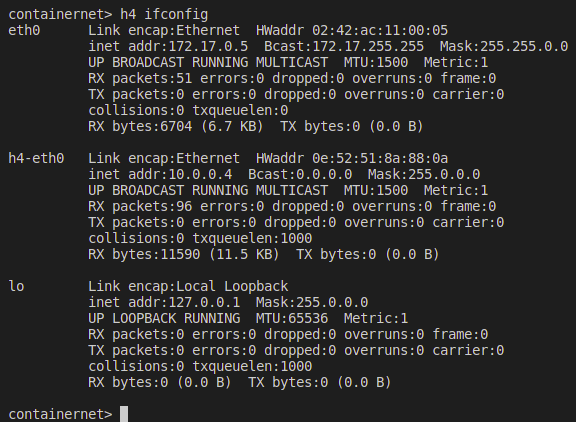
\includegraphics[width=0.45\textwidth]{Imagenes/item01_h4_ifconfig.png}}
    \caption{Configuración de redes para los host}
    \label{fig:item01pinghost}
\end{figure}

\noindent
Ingresamos a las terminales de cada host, a través de la opción de xterm en la consola de containernet (mininet). Una vez ingresado, corroboramos la conexión entre hosts mediante el uso de 10 pings entre h1 y h2, como en h1 y h3. Con estas muestras es posible determinar el delay correspondiente a los enlaces, puesto que la conexión de h1-h2 solamente atraviesa el switch s1 que no posee ningún tipo de delay asociado, donde se observa que el tiempo promedio de ida y vuelta es de 1,483 milisegundos. Mientras que la conexión entre h1-h3, atraviesa el enlace s2-s3 que posee un delay de 15 milisegundos, tomando en cuenta el viaje de ida y vuelta, se puede verificar que efectivamente se está realizando el retardo correspondiente dado que se observa que el promedio de tiempo es de 30,797 milisegundos.\newline

\begin{figure}[H]
\centering
\subfloat[Ping realizado de h1 a h2]{
\label{CDF1}
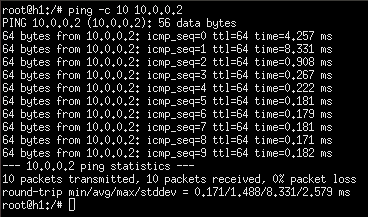
\includegraphics[width=0.45\textwidth]{Imagenes/item01_ping_h1-h2.png}}
\subfloat[Ping realizado de h1 a h3]{
\label{CDF2}
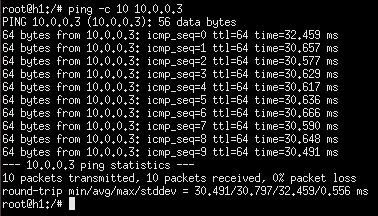
\includegraphics[width=0.45\textwidth]{Imagenes/item01_ping_h1-h3.png}}
\caption{Ejecución de pings}
\label{fig:item01pinghost}
\end{figure}

\noindent
Para cada una de estas muestras, fue necesario iniciar una captura en wireshark con tal de corroborar el intercambio de paquetes a través de la red, tanto de ICMP como de paquetes ARP como se muestra en las imágenes a continuación.

\begin{figure}[H]
    \centering
    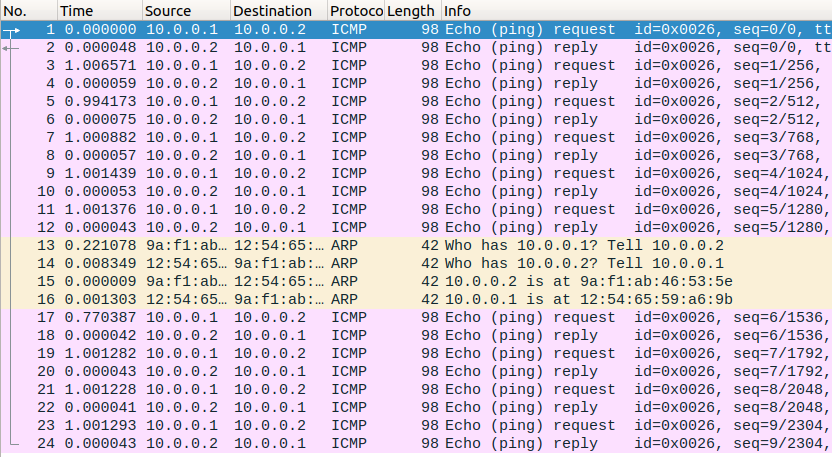
\includegraphics[width=0.7\textwidth]{Imagenes/item01_ping_h1-h2_Wireshark.png}
    \caption{Captura de Wireshark - Ping entre h1 y h2}
    \label{fig:item01_h1_h2_Wire}
\end{figure}

\begin{figure}[H]
    \centering
    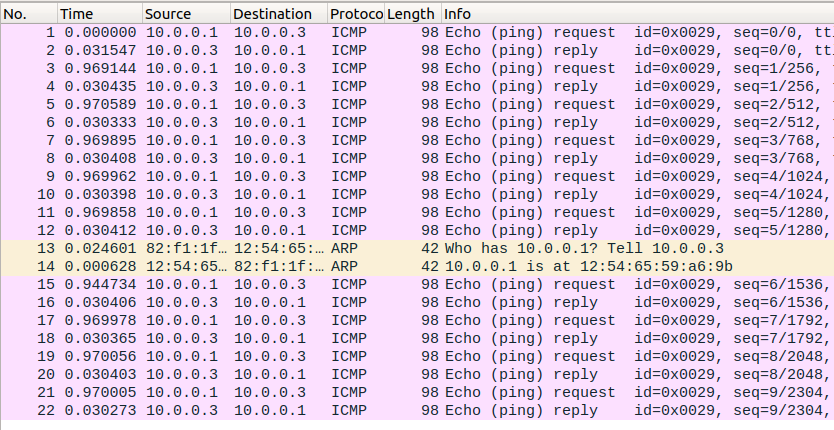
\includegraphics[width=0.7\textwidth]{Imagenes/item01_ping_h1-h3_Wireshark.png}
    \caption{Captura de Wireshark - Ping entre h1 y h3}
    \label{fig:item01_h1_h3_Wire}
\end{figure}


\begin{multicols}{2}

\noindent
Una vez probada la conectividad de la red, se pone a prueba el enlace que conecta los switches s3 y s4 respectivamente, con el fin de lograr medir la configuración de retardos establecida a través del software. Es necesario comprobar el porcentaje de pérdidas del enlace establecido, para ello resulta necesario tomar una muestra lo suficientemente grande de pings entre los hosts h3 y h4, de tal forma de determinar un intervalo de confianza con 95\%. \newline

\noindent
Como se observa en la figura \ref{fig:ping_10000}, se realiza un ping con una cantidad de 10000 request, cuyos resultados se describan en la siguiente tabla.\newline


\columnbreak

\begin{figure}[H]
    \centering
    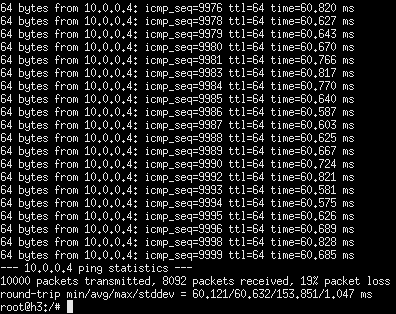
\includegraphics[width=0.8\linewidth]{Imagenes/ping_10000.png}
    \caption{Resultados obtenidos del ping}
    \label{fig:ping_10000}
\end{figure}

\end{multicols}

\begin{table}[H]
\centering
    \resizebox{0.6\linewidth}{!}{%
    \begin{tabular}{|c|c|c|c|c|}
    \hline
    \rowcolor[HTML]{DAE8FC} 
    {\color[HTML]{000000} \textbf{Mínimo}} &
      {\color[HTML]{000000} \textbf{Promedio}} &
      {\color[HTML]{000000} \textbf{Máximo}} &
      {\color[HTML]{000000} \textbf{Desviación Estándar}} \\ \hline
    60,121 & 60,632 & 153,851 & 1,047 \\ \hline
    \end{tabular}
    }
    \caption{hola}
\end{table}

\noindent
A partir de los datos del cuadro anterior, específicamente el promedio y la desviación estándar, es posible calcular el intervalo de confianza el cual corresponde a 60,61 [ms] como límite inferior y 60,65 [ms] como límite superior.

\subsection{Actividad 02}

\begin{multicols}{2}

\noindent
A través de la misma topología de red anterior, se va a implementar un servicio de http en el host h1, a la vez que el host h2 va a realizar una petición al servicio a través del comando wget. Para el caso del servidor se usa un módulo integrado de python, tanto cliente como servidor son llevados a cabo a través de la consola de containernet mediante las líneas de comando.\newline

\begin{minted}[frame=lines, fontsize=\footnotesize,bgcolor=white,linenos]{bash}
containernet> h1 python3 -m http.server 80 &
containernet> h2 wget -O - h1
\end{minted}

\noindent
El primer comando, levantará el servidor en el equipo h1 de manera asíncrona a través del módulo http.server, habilitando el directorio actual donde se ejecuta (en este caso la carpeta raíz del sistema /) a través de html. Mientras que el segundo comando, wget se utiliza para descargar archivos a través de internet (http), particularmente la solicitud va dirigida a la ip del host h1 y la opción -O omite la descarga del archivo con la finalidad de desplegar su contenido en la propia terminal. \newline

\noindent
El tráfico de conexión entre ambos host logra visualizarse a través de wireshark. En la figura \ref{fig:item02_wget_terminal} a continuación se observan los paquetes filtrados por las ip’s correspondiente a los hosts en la figura \ref{fig:item02_wget_wireshark}, donde se visualiza que el paquete N° 4 preseleccionado posee el requerimiento GET en HTTP. \newline

\columnbreak

\begin{figure}[H]
    \centering
    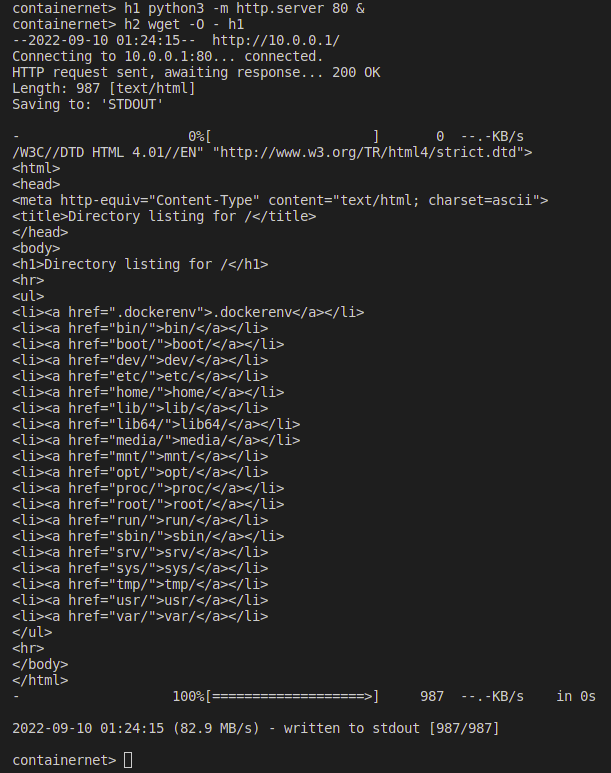
\includegraphics[width=\linewidth]{Imagenes/item02_GET_TERMINAL.png}
    \caption{Solicitud mediante el comando wget}
    \label{fig:item02_wget_terminal}
\end{figure}

\end{multicols}

\begin{figure}[H]
    \centering
    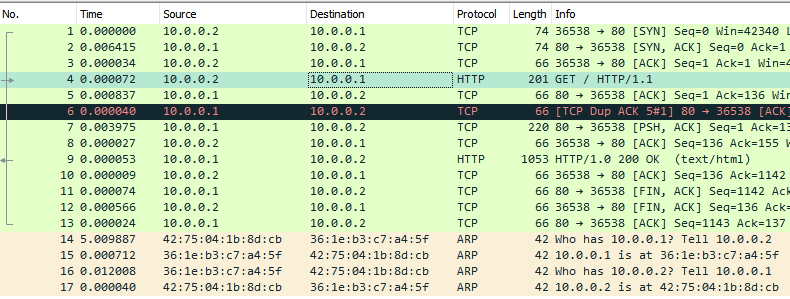
\includegraphics[width=\linewidth]{Imagenes/item02_GET.png}
    \caption{Tráfico de red de solicitud GET a través de Wireshark}
    \label{fig:item02_wget_wireshark}
\end{figure}

\noindent
Cabe recalcar, que si se realiza nuevamente la prueba tomando en consideración la interfaz any, se logra observar que los equipos de la red envían más paquetes a través de la red. Tras filtrar y observar con mayor detalle el comportamiento del tráfico a través de las diversas interfaces, se puede concluir que el tráfico corresponde a la interfaz de Loopback. Esta interfaz tiene como funcionalidad establecer una conexión de red virtual, la cual muy posiblemente es utilizada por el controllador de containernet (mininet) para el uso de la propia red virtual.
\newline



\begin{multicols}{2}

\begin{figure}[H]
    \centering
    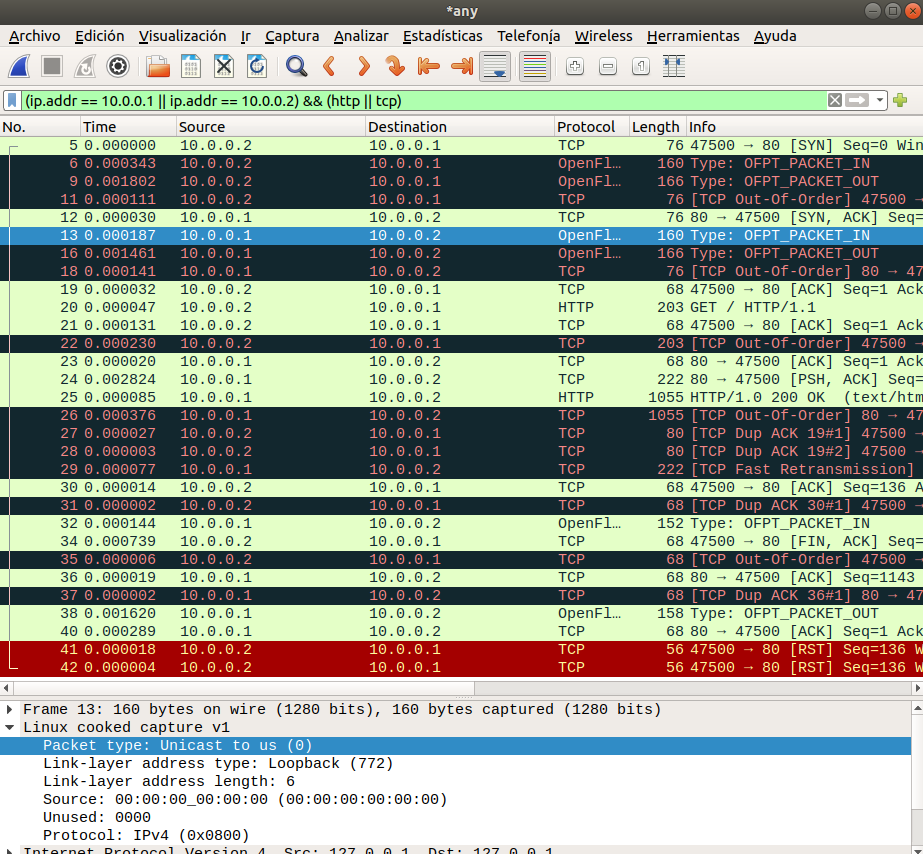
\includegraphics[width=\linewidth]{Imagenes/item02_GET_interface_any.png}
    \caption{Solicitud mediante el comando wget}
    \label{fig:item02_any}
\end{figure}

\columnbreak

\begin{figure}[H]
    \centering
    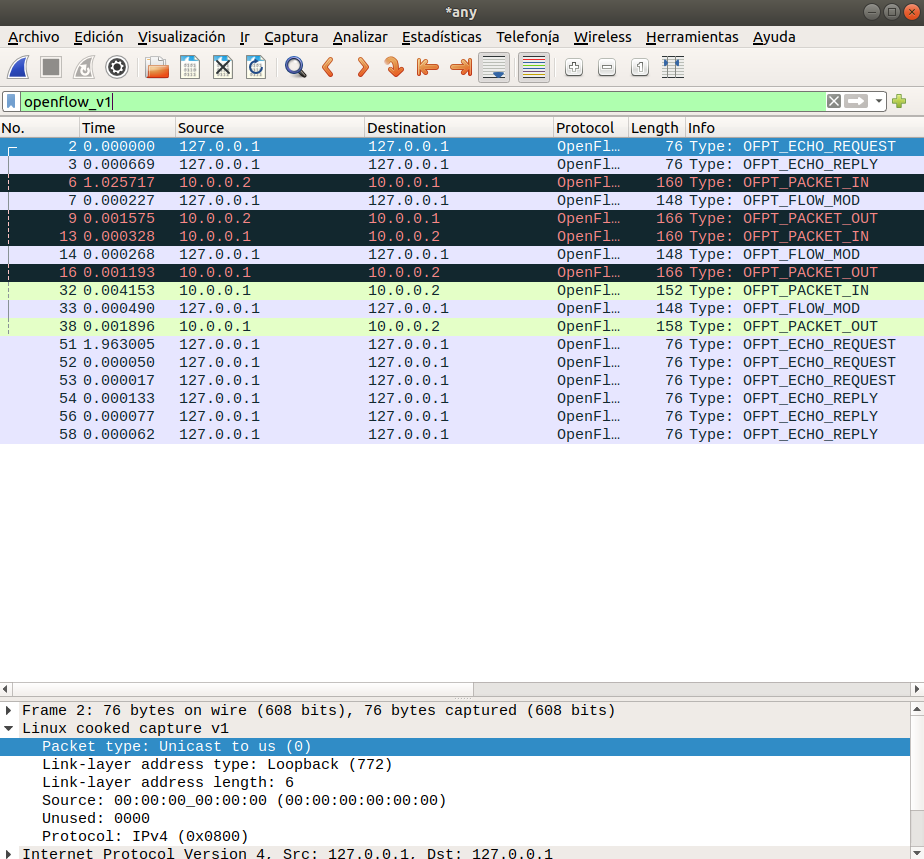
\includegraphics[width=\linewidth]{Imagenes/loopback.png}
    \caption{Solicitud mediante el comando wget}
    \label{fig:item02_loopback}
\end{figure}

\end{multicols}

\newpage

\subsection{Actividad 03}

La siguiente actividad consiste en la implementación de una topología de red tree mediante el protocolo NAT. Para realizar esto último, mininet nos brinda un archivo predeterminado ubicado en la siguiente ruta /containernet/examples/nat.py , el cual puede ser ejecutado con el siguiente comando dentro del contenedor.

\begin{minted}[frame=lines, fontsize=\footnotesize,linenos]{bash}
#!/bin/bash
sudo python3 /containernet/examples/nat.py 
\end{minted}

Se comprueba que cada host de la red NAT tenga acceso a algún sitio público de internet como Facebook. Para corroborar esto último, se efectúa unos pings hacia el sitio web de Facebook en cada uno de los hosts, como se observa en las imágenes a continuación.

\begin{figure}[H]
    \centering
    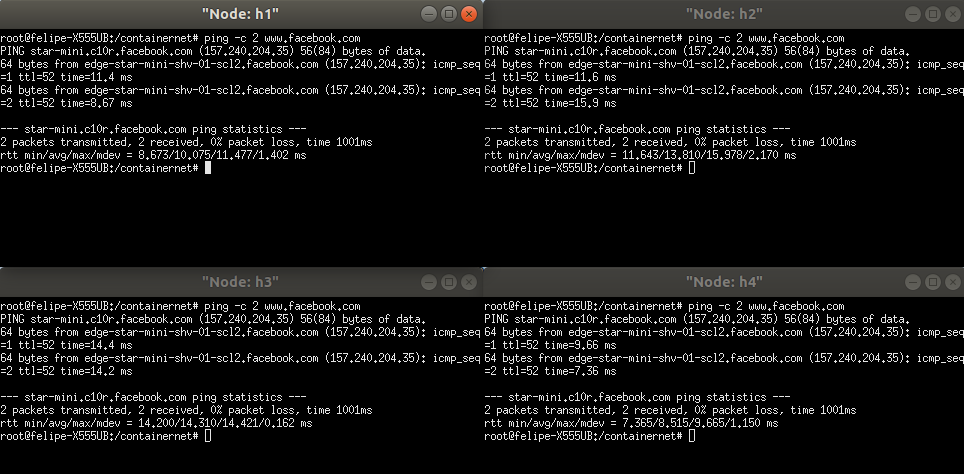
\includegraphics[width=0.9\linewidth]{Imagenes/item03_ping_facebook_terminal.png}
    \caption{Solicitudes de ping a través de xterm}
    \label{fig:item03_piing_xterm}
\end{figure}

\begin{figure}[H]
    \centering
    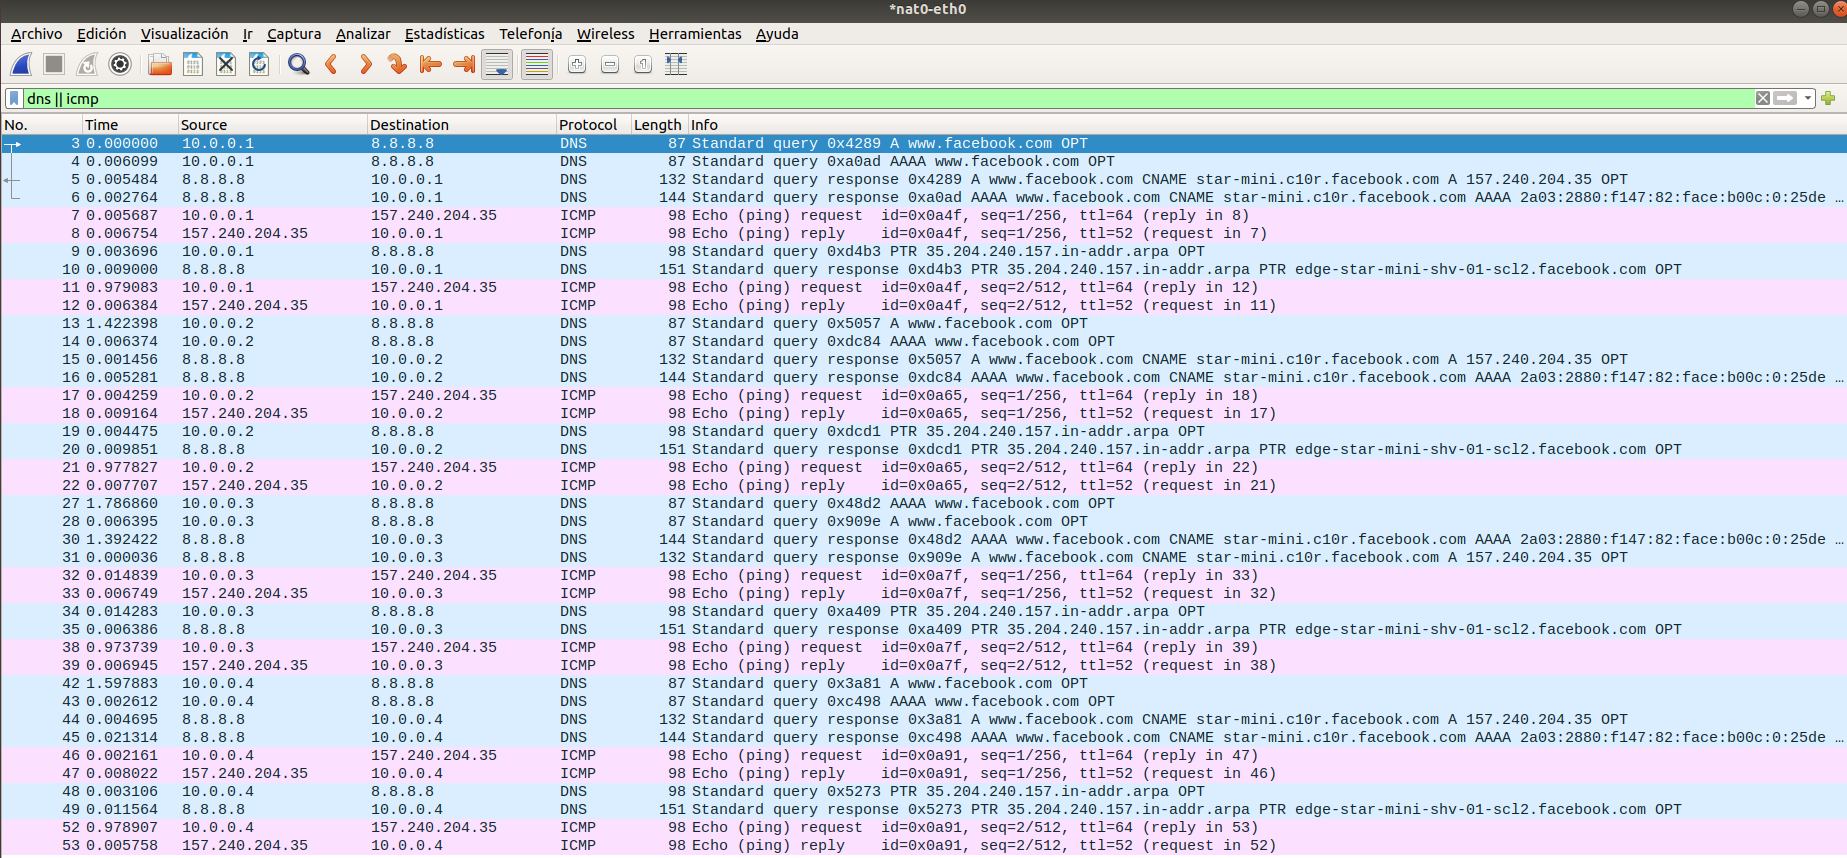
\includegraphics[width=\linewidth]{Imagenes/item03_ping_facebook.png}
    \caption{Tráfico de red generado por los pings a Facebook}
    \label{fig:item03_ping_wireshark}
\end{figure}

Finalmente, montamos el mismo servicio de python usado en la actividad anterior, accediendo al sitio web del host utilizado a través de la IP del mismo, como se observa en la imagen a continuación.

\begin{figure}[H]
    \centering
    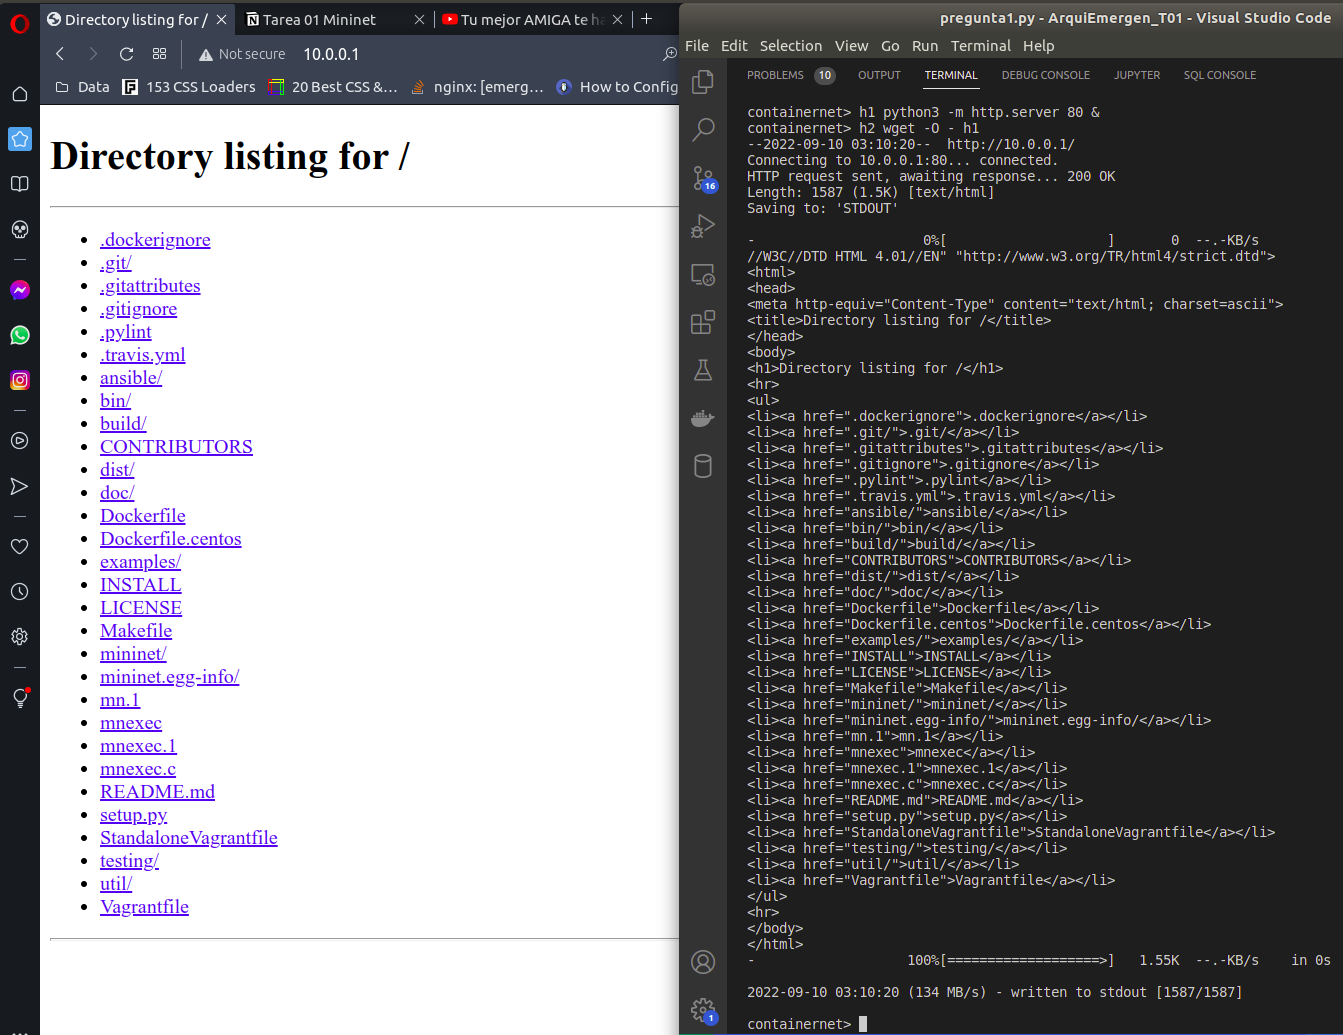
\includegraphics[width=0.9\linewidth]{Imagenes/item03_Directory.png}
    \caption{Acceso al servicio http del host h1 a través de navegador Opera en la máquina local}
    \label{fig:item03_direcotry}
\end{figure}

\begin{figure}[H]
    \centering
    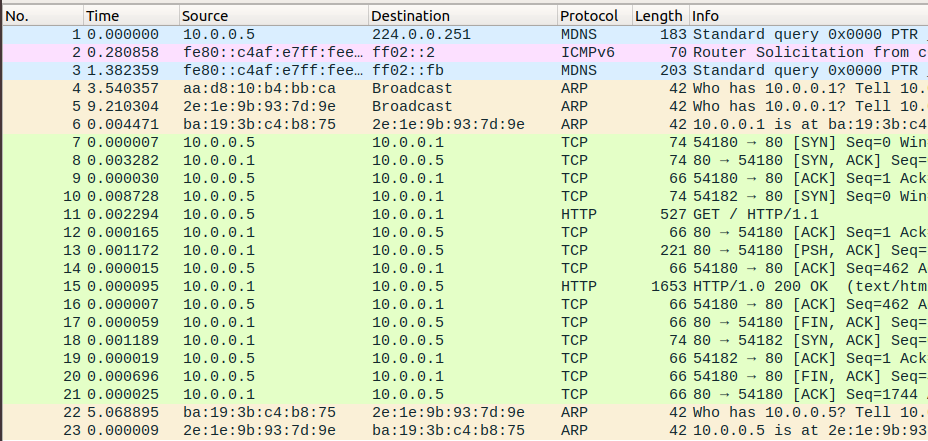
\includegraphics[width=0.9\linewidth]{Imagenes/item03_GET_Wireshark.png}
    \caption{Captura de tráfico de ingreso por navegador}
    \label{fig:item03_directory_wireshark}
\end{figure}

Como se logra observar en la captura de wireshark, las ip de los host involucrados corresponden a 10.0.0.1 (host donde se encuentra el servicio http) y 10.0.0.5 (correspondiente al NAT), dado que la configuración de red NAT habilita la asignación de direcciones tanto internas como externas, es normal que la máquina local en vez de comunicarse con el servicio con su propia ip, lo haga a través del dirección de NAT en la topología virtual. Considerando que la captura es realizada a través de la interfaz NAT dispuesta en la red, es normal que en la muestra de tráfico no se vea reflejado los paquetes de solicitud realizados por el host h2 a través de la terminal de containernet mostrado en la figura \ref{fig:item03_direcotry} y solamente se vea las solicitudes realizadas desde el exterior de la red, como lo es el navegador de Opera.


\subsection{Actividad 4}

Para esta actividad se implementa una topología diferente a la anterior, correspondiente a la figura \ref{fig:item04_net}. Se analiza el enlace entre los host de Chile y Australia mediante el comando iperf, el cual es una herramienta de red de código abierto utilizada para medir el rendimiento de una red. Se puede utilizar para probar el funcionamiento de canales a través de TCP y UDP.

\begin{figure}[H]
    \centering
    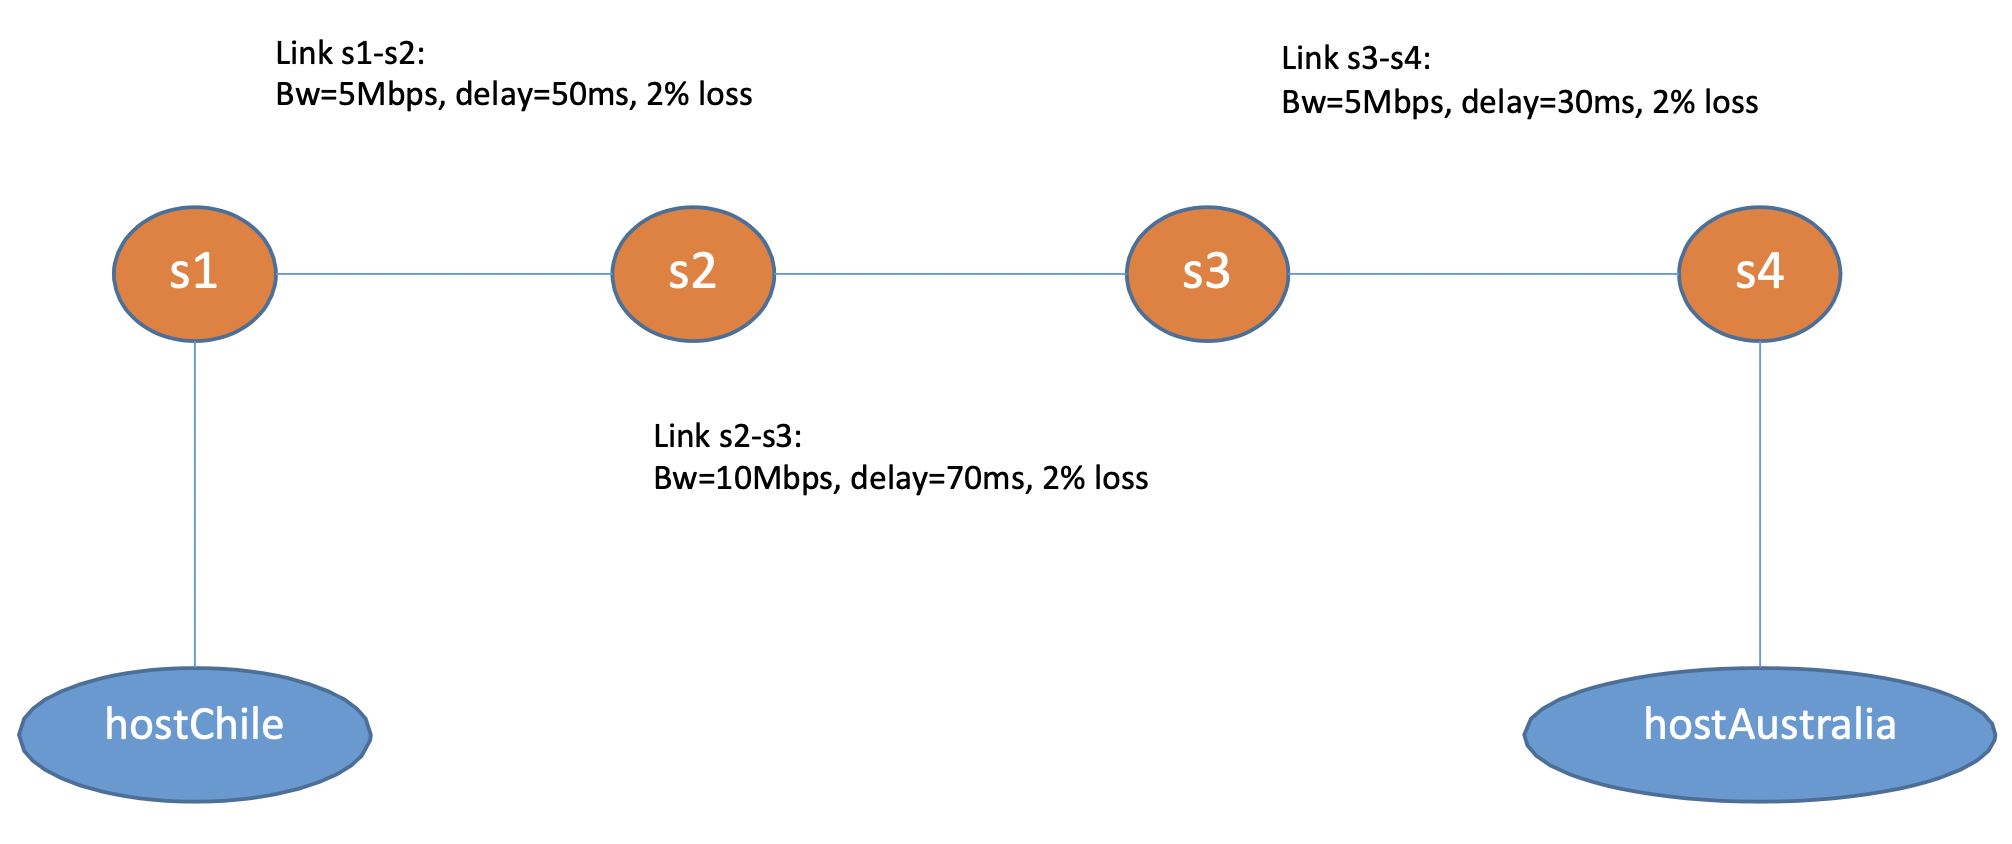
\includegraphics[width=0.7\linewidth]{Imagenes/item04_network.png}
    \caption{Topología de red - Actividad 04}
    \label{fig:item04_net}
\end{figure}

\noindent
Como se observa en la figura \ref{fig:item04_iperf} y \ref{fig:item04_iperf02}, el comando iperf los brinda tanto los intervalos, la cantidad de datos transferidos y el ancho de banda del canal de transporte TCP. A través de estos, es posible medir el impacto que tiene las pérdida en los enlaces entre los hosts de Chile y Australia, aún considerando que la red corresponde a una topología serial, el ancho de banda de menor alcance corresponde a 5 Megabytes por segundo. Pero como se logra observar en los resultado, tanto la pérdida como el delay generan que la conexión establecida posea un ancho de banda alrededor de 240 Kilobytes por segundo aproximadamente.


\begin{figure}[H]
    \centering
    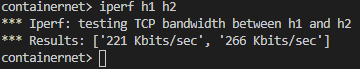
\includegraphics[width=0.6\linewidth]{Imagenes/iperf.png}
    \caption{Ejecución de iperf a través de containernet}
    \label{fig:item04_iperf}
\end{figure}

\begin{figure}[H]
    \centering
    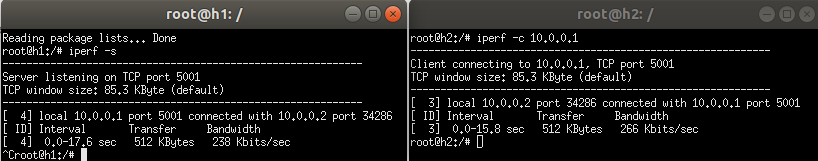
\includegraphics[width=1\linewidth]{Imagenes/iperf2.png}
    \caption{Ejecución de iperf cliente/servidor}
    \label{fig:item04_iperf02}
\end{figure}

Una vez caracterizado el enlace, se procede a realizar una descarga de un archivo entre hosts a través de la red. Para realizar esto, ambos host se comunicarán bajo una arquitectura de cliente/servidor. El equipo h2 va a contener un servidor FTP, el cual brindará acceso remoto sobre las carpetas de usuarios creados dentro de la máquina. Mientras que el equipo h1, instalará un cliente ftp para acceder a las carpetas de usuarios brindados por el servidor FTP remoto, con la finalidad de descargar algún archivo disponible y examinar de manera analítica el tráfico generado entre el host h1 y el switch s1. 

\subsubsection*{Servidor}

Se crea a un usuario dentro de la máquina con nombre de usuario y contraseña admin, generando su carpeta correspondiente en el directorio /home . Luego en la carpeta de este usuario, se genera una imagen en formato png de 10 Mb de tamaño a través del comando fallocate, como se observa en la figura \ref{fig:item04_servidor}. \newline

\noindent
Luego instalamos e instanciamos el servicio de FTP a través de las siguientes líneas de comando. Donde también se verifica que el servicio se encuentre operativo a través del puerto 21, como se muestra en la figura \ref{fig:item04_port21}.\newline

\begin{multicols}{2}

\begin{figure}[H]
    \centering
    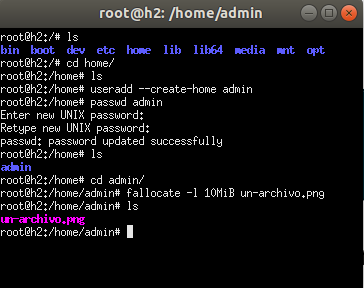
\includegraphics[width=0.9\linewidth]{Imagenes/item04_user_and_file.png}
    \caption{Creación de usuarios y archivo}
    \label{fig:item04_servidor}
\end{figure}
\hfill
\columnbreak
\hfill
\begin{minted}[frame=lines, fontsize=\footnotesize,bgcolor=white,linenos]{bash}
# Instalación
apt update
apt install -y ftpd

# Despliegue
inetd

# Verificación - Puerto 21
netstat -tulp
\end{minted}
\hfill
\begin{figure}[H]
    \centering
    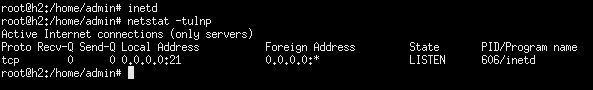
\includegraphics[width=\linewidth]{Imagenes/item04_ftp_service.png}
    \caption{Verificación del servicio ftp - Port 21}
    \label{fig:item04_port21}
\end{figure}

\end{multicols}

\subsubsection*{Cliente}




\begin{multicols}{2}

Ingresamos al directorio /tmp donde se iniciará la descarga del documento a través de consola. Luego se instala un cliente FTP y se conecta al servicio iniciado por el host h2 a través de su ip 10.0.0.2 . Una vez abierto el cliente FTP, nos autenticamos con las credenciales del usuario admin creado previamente en el servidor. Finalmente, cuando se establezca la conexión, ejecutamos el comando GET un-archivo.png, este iniciará la descarga del documento alojado en la carpeta del usuario admin proveniente del servidor, el cual fue creado pasos atrás. Los pasos descritos se pueden observar en la figura \ref{fig:item04_download}, al igual que la captura de paquetes a través de Wireshark mostrada en la figura \ref{fig:item04_download_wireshark}.


\columnbreak

\begin{figure}[H]
    \centering
    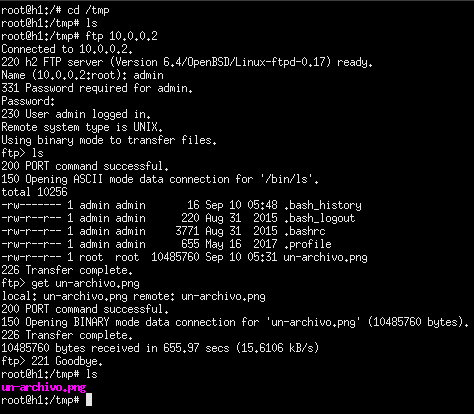
\includegraphics[width=\linewidth]{Imagenes/item04_ftp_client_download.png}
    \caption{Descarga del archivo}
    \label{fig:item04_download}
\end{figure}


\end{multicols}

\begin{figure}[H]
    \centering
    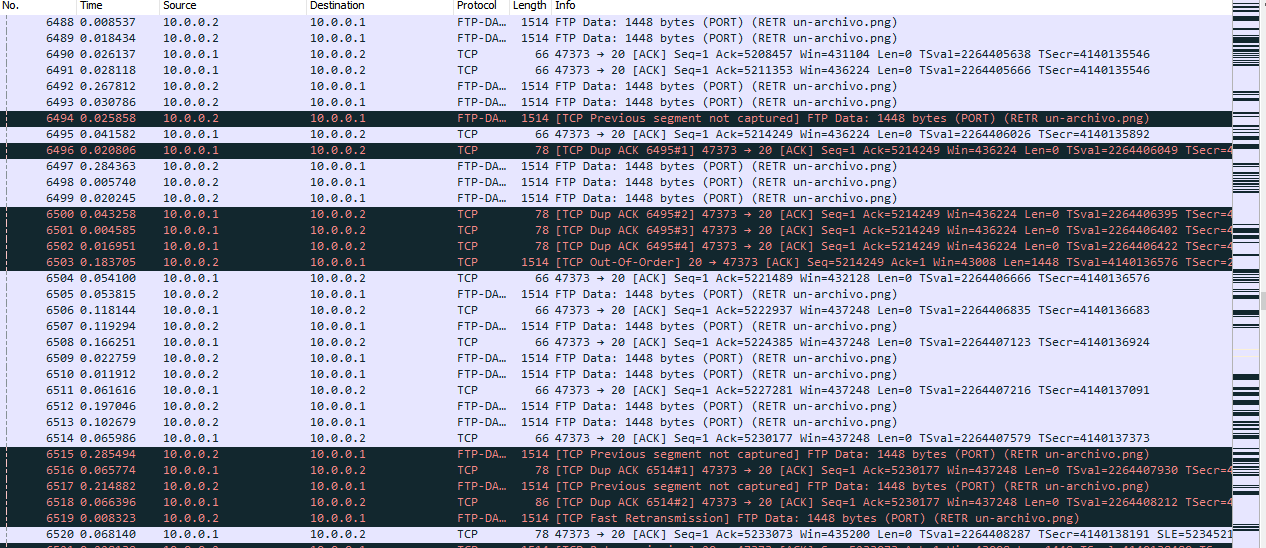
\includegraphics[width=\linewidth]{Imagenes/ftp_traffic.png}
    \caption{Tráfico FTP obtenido por la descarga del archivo}
    \label{fig:item04_download_wireshark}
\end{figure}


\subsubsection*{Análisis}



\begin{tcolorbox}[enhanced,frame style image=blueshade.png,
  opacityback=0.75,opacitybacktitle=0.25,
  colback=blue!5!white,colframe=blue!75!black,
  title=¿Qué problemas se puede observar en la transmisión TCP de paquetes? ¿Por qué se producen? ¿Cómo resuelve TCP este problema?]
  
  
  En el tráfico medido a través de Wireshark, como se observa en la figura \ref{fig:item04_download_wireshark}, existe una gran cantidad de paquetes perdidos o retrasos en la transmisión de ciertos segmentos, lo que resulta crucial para el protocolo de transporte de TCP, puesto que dentro de sus objetivos también es necesario entregar la información en un orden establecido, lo que provoca una mayor demora en el tiempo total para completar la descarga del archivo en cuestión.\newline
  
  \noindent
  La principal causa es la propia inestabilidad del canal, más específicamente las de los enlaces entre los switch, dado que el alto delay junto al bajo ancho de banda de cada uno de estos, incrementa acumulativamente el riesgo de que ocurra alguna pérdida o retraso en la transmisión, volviendo al canal un medio en extremo inestable y poco predecible. Por estos motivos se observa una gran cantidad de fallas en la comunicación entre el cliente y el servidor. \newline
  
  \noindent
  Para resolver esta problemática, el propio protocolo TCP tiene ciertas políticas, como la retransmisión de paquetes o duplicaciones de ACK entre muchas otras, para mantener así una cohesión de la información transmitida, a través de nuevos tipos de mensajes o flags que mantienen a ambos equipos coordinados en la manera y orden de transmisión de datos, aunque estos mismos mecanismos son los que provocan que se demora en gran medida el tiempo de descarga, llegando a demorar alrededor de 6 minutos con 55 segundos. 
  
  
  

\end{tcolorbox}


\begin{tcolorbox}[enhanced,frame style image=blueshade.png,
  opacityback=0.75,opacitybacktitle=0.25,
  colback=blue!5!white,colframe=blue!75!black,
  title=¿Sería conveniente usar un enlace UDP para la transferencia de archivos en este tipo de enlace?]
  
  A diferencia de TCP, el protocolo UDP no se preocupa en mantener una conexión o transmisión ordenadas de los datos, al igual que tampoco coordina entre ambos equipos el correcto recibimiento de los segmentos enviados. Por esto mismo el protocolo UDP es recomendable usarlo en contexto donde se requiera una transmisión en tiempo real de datos, como pueden ser distintas aplicaciones de streaming o big data y no para transferencia de archivos, puesto que no posee estas cualidades para verificar el correcto envío de información que si posee TCP. \newline 
  
  \noindent
  Aún así, cabe recalcar que el protocolo FTP al proveer estos mecanismos genera un problema aún más grande, debido a que incrementa considerablemente la congestión de la propia red a causa de la inestabilidad de los enlaces. Las consecuencias de este canal tan débil sumado a las políticas del protocolo se pueden ver reflejadas en la información especializada de Wireshark mostrada en la figura \ref{fig:item04_download_wireshark_info}, donde más de 5000 paquetes (cerca del 40\% de la muestra total) corresponden a errores de transmisión o corrección por TCP, lo cual incrementa en gran medida la latencia y congestión de la red.\newline
  
  \noindent
  Finalmente, se puede concluir que si bien TCP está diseñado para la transferencia correcta de archivos, no cumple o satisface todas las necesidades para la arquitectura de red que se está simulando. Debido a esto, y la necesidad de una red con el tipo de enlaces con baja estabilidad, se puede determinar que para estas situaciones resulta mucho más conveniente utilizar el protocolo UDP, para realizar este tipo transferencias con enlaces de estas características.
  

\begin{figure}[H]
    \centering
    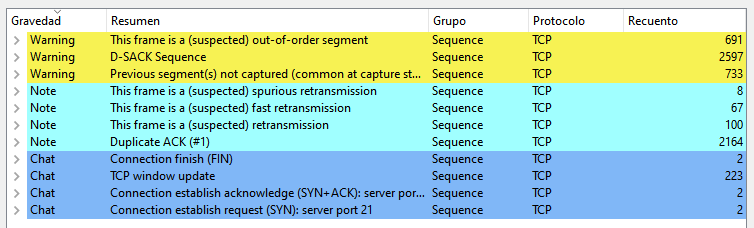
\includegraphics[width=\linewidth]{Imagenes/ftp_info.png}
    \caption{Información especializada de Wireshark}
    \label{fig:item04_download_wireshark_info}
\end{figure}

\end{tcolorbox}







\end{document}
